\documentclass[a4paper,12pt,oneside]{article}
%\usepackage[portuguese]{babel}
%\usepackage[latin1]{inputenc}
\usepackage[utf8]{inputenc}
\usepackage[T1]{fontenc}
\usepackage{fancyhdr}
\usepackage{pdfpages} 
\usepackage{mdwlist}
\usepackage{bm}
\usepackage{blindtext}
\usepackage{array}
\usepackage{multicol}
\usepackage{multirow}
\usepackage{mdwlist}
\usepackage{enumitem}
\usepackage[numbers]{natbib}
\usepackage{url} 
\usepackage{graphicx}
\usepackage{caption}    
\usepackage{amsmath}
\usepackage{amsthm}
\usepackage{amsfonts}
\usepackage{mathrsfs}
\usepackage{amssymb}
\usepackage{mdframed}
\usepackage{xcolor}
\usepackage{fourier-orns}
\usepackage{geometry}
\usepackage{parskip}
\usepackage{listings}
\usepackage{setspace}
\usepackage{imakeidx}
\usepackage{makeidx}
\usepackage{authblk} 
\usepackage{setspace} 
\usepackage{etoolbox}
\usepackage[
            pdftex
            ,plainpages=false
            ,pdfpagelabels
            ,pagebackref = false
            ,hyperindex
            ,breaklinks=true 
            ,colorlinks=true 
            ,citecolor=black 
            ,linkcolor=black
            ,urlcolor=black
            ,filecolor=black
            ,bookmarksopen=true
            ]{hyperref}
%%%%%%%%%%%%%%%%%%%%%%%%%%%%%%%%%%%%%%%%%%%%%%%%%%%%%%%%%%%%%%%%%%%%%%%
\makeatletter
\renewenvironment{abstract}{
    \if@twocolumn
        \section*{Abstract}
    \else
        \small
        \begin{center}
            {\bfseries \abstractname\vspace{-.5em}\vspace{\z@}}%
        \end{center}
        \noindent
    \fi
}
%{\par\vspace{1.5em}\noindent\hrulefill\par} 
\makeatother
%%%%%%%%%%%%%%%%%%%%%%%%%%%%%%%%%%%%%%%%%%%%%%%%%%%%%%%%%%%%%%%%%%%%%%%
\lstset{
  language=Python,
	basicstyle = \fontsize{10}{12}\ttfamily%\small
  keywordstyle=\color{blue},
  commentstyle=\color{green!60!black},
  stringstyle=\color{red},
  showstringspaces=false,
  breaklines=true,
  frame=single,
  numbers=left,
  numberstyle=\tiny\color{gray},
  captionpos=b,
  escapeinside={(*@}{@*)} % If you need to include LaTeX within your code
}
%%%%%%%%%%%%%%%%%%%%%%%%%%%%%%%%%%%%%%%%%%%%%%%%%%%%%%%%%%%%%%%%%%%%%%%
\textheight 9in  
\topmargin -.5in   
\def\baselinestretch{1.06}
\textwidth 6.6in 
\oddsidemargin 0in 
\evensidemargin 0in
\geometry{left=25mm,right=25mm,top=25mm,bottom=25mm}
\addtocontents{toc}{\protect\setcounter{tocdepth}{2}}
\numberwithin{equation}{section}
%%%%%%%%%%%%%%%%%%%%%%%%%%%%%%%%%%%%%%%%%%%%%%%%%%%%%%%%%%%%%%%%%%%%%%%%%%%%
\lstset{
  language=Python,
	basicstyle = \fontsize{10}{12}\ttfamily%\small
  keywordstyle=\color{blue},
  commentstyle=\color{green!60!black},
  stringstyle=\color{red},
  showstringspaces=false,
  breaklines=true,
  frame=single,
  numbers=left,
  numberstyle=\tiny\color{gray},
  captionpos=b,
  escapeinside={(*@}{@*)} % If you need to include LaTeX within your code
}
%%%%%%%%%%%%%%%%%%%%%%%%%%%%%%%%%%%%%%%%%%%%%%%%%%%%%%%%%%%%%%
\DeclareMathOperator{\sech}{sech}
\newcommand{\sen}{\mathrm{sen}}
\newcommand{\dd}{\mathrm{d}}
\newcommand{\keywords}[1]{\textbf{\textit{keywords:}} #1}
\newcommand{\palavraschave}[1]{\textbf{\textit{palavras-chave:}} #1}
\newcommand{\EE}{\mathbf{e}}
\newcommand{\RR}{\mathrm{R}}
\newcommand{\GG}{\mathbf{G}}
\newcommand{\TT}{\mathrm{T}}

\def\be{\begin{equation}}
\def\ee{\end{equation}}
\def\ni{\noindent}

\addtocontents{toc}{\protect\setcounter{tocdepth}{2}}
\numberwithin{equation}{section}
\setlength{\parindent}{1cm}

\def\NAT@def@citea{\def\@citea{\NAT@separator}}%
%%%%%%%%%%%%%%%%%%%%%%%%%%%%%%%%%%%%%%%%%%%%%%%%%%%%%%%%%%%%%%%%%%%%%%%%%%%%
% Number exercises within subsections
\newtheorem{exercise}{Exercise}[section]
\newtheorem{definition}{Definition}
\newtheorem{example}{Example}
\newtheorem{corollary}{Corollary}

%%%%%%%%%%%%%%%%%%%%%%%%%%%%%%%%%%%%%%%%%%%%%%%%%%%%%%%%%%%%%%%%%%%%%%%%%%%%
\makeindex

\title{A Recreational Mathematical Geometry Note on Arc Lengths in Chains of Tangent Circles}

\author[1]{Osvaldo L. Santos-Pereira 
\thanks{olsp@if.ufrj.br}
\thanks{\href{https://orcid.org/0000-0003-2231-517X}{ORCID: 0000-0003-2231-517X}}}
\affil[1]{Graduate Program in Multidisciplinary Applied Physics (PPGMFA) Physics Institute Universidade Federal do Rio de Janeiro (UFRJ)}
\date{\today}

\begin{document}
\maketitle

\begin{abstract}
\ni
This text presents a solution to a plane geometry problem and its generalization. The problem is taken from Volume 9 of the collection \textit{Fundamentos da Matemática Elementar}, a classical Brazilian collection of elementary mathematics books aimed at high school students, composed of 11 volumes. Volume 9 is devoted to plane geometry and contains several problems that, despite their elementary formulation, offer valuable opportunities for mathematical reasoning.
\end{abstract}

\noindent\textbf{Keywords:} recreational mathematics; plane geometry; tangent circles; circular arcs; arc length; explementary angle

\section{Introduction}

Euclidean plane geometry is one of the most suitable subjects for the development of mathematical reasoning, especially for early-stage students. Its objects are visually intuitive, yet its conclusions require precise definitions, logical organization, and rigorous proof. In this context, students are naturally led to distinguish between what appears to be true in a figure and what can be demonstrated from axioms, theorems, and previously established results. Problems involving lines, angles, circles, polygons, tangency, and congruence provide a rich environment for practicing proof techniques such as direct proof, proof by contradiction, auxiliary constructions, decomposition of figures, and generalization from particular configurations. For this reason, plane geometry occupies a privileged position in mathematical education: it connects visual intuition with deductive reasoning, showing that mathematics is not merely the computation of numerical answers, but the disciplined construction of arguments.

\ni
The problem analyzed here concerns the length of a curve formed by successive arcs of tangent circles. It is taken from Problem 737 of Volume 9 of the collection \textit{Fundamentos da Matemática Elementar}, in the edition used as reference in this work. Since this is an older edition of the book, the same problem may not appear with the same numbering, or may not appear at all, in newer editions.

\ni
Although the computation is simple, the exercise illustrates an important feature of mathematical thinking: the ability to identify the geometric structure behind a particular configuration and then generalize the result to an arbitrary one. In this sense, the problem naturally belongs to recreational mathematics, where elementary problems serve as a gateway to abstraction, pattern recognition, and generalization. The problem statement is as follows. Fig.\,\ref{fig:geometric-configuration} is also part of the statement.

\ni
\textbf{Problem.} \textit{If the angles at the vertices $O_1, O_2, O_3, O_4$ and $O_5$ measure, respectively, $90^\circ$, $72^\circ$, $135^\circ$, $120^\circ$ and $105^\circ$, and the radii of the circles centered at these vertices measure, respectively, $18\,\mathrm{cm}$, $35\,\mathrm{cm}$, $24\,\mathrm{cm}$, $36\,\mathrm{cm}$ and $48\,\mathrm{cm}$, determine the length of the curve $AB$.}

\begin{figure}[ht]
    \centering
    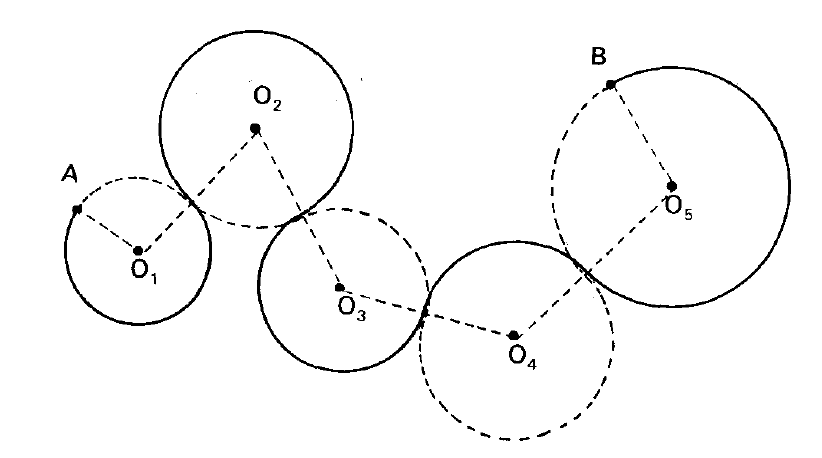
\includegraphics[width=0.8\textwidth]{article-image.png}
    \caption{Original image that is also the statement of the problem in Ref.\,\cite{dolce-pompeo}, it presents the geometric configuration of the line $AB$, formed by successive arcs of tangent circles.}
    \label{fig:geometric-configuration}
\end{figure}

\begin{proof}[\textbf{Solution}]

\ni
The exercise analyzed proposes determining the length of a line formed by successive arcs of tangent circles, with known angles and radii. As stated in the problem, five centers, $O_1, O_2, O_3, O_4, O_5$, are given, each associated with a specific central angle and radius. The objective is to determine the total length of the line $AB$, constructed from the outer arcs of these circles. Before delving into the solution of this problem, we shall review a useful definition regarding circular arcs.

\begin{figure}[ht]
    \centering
    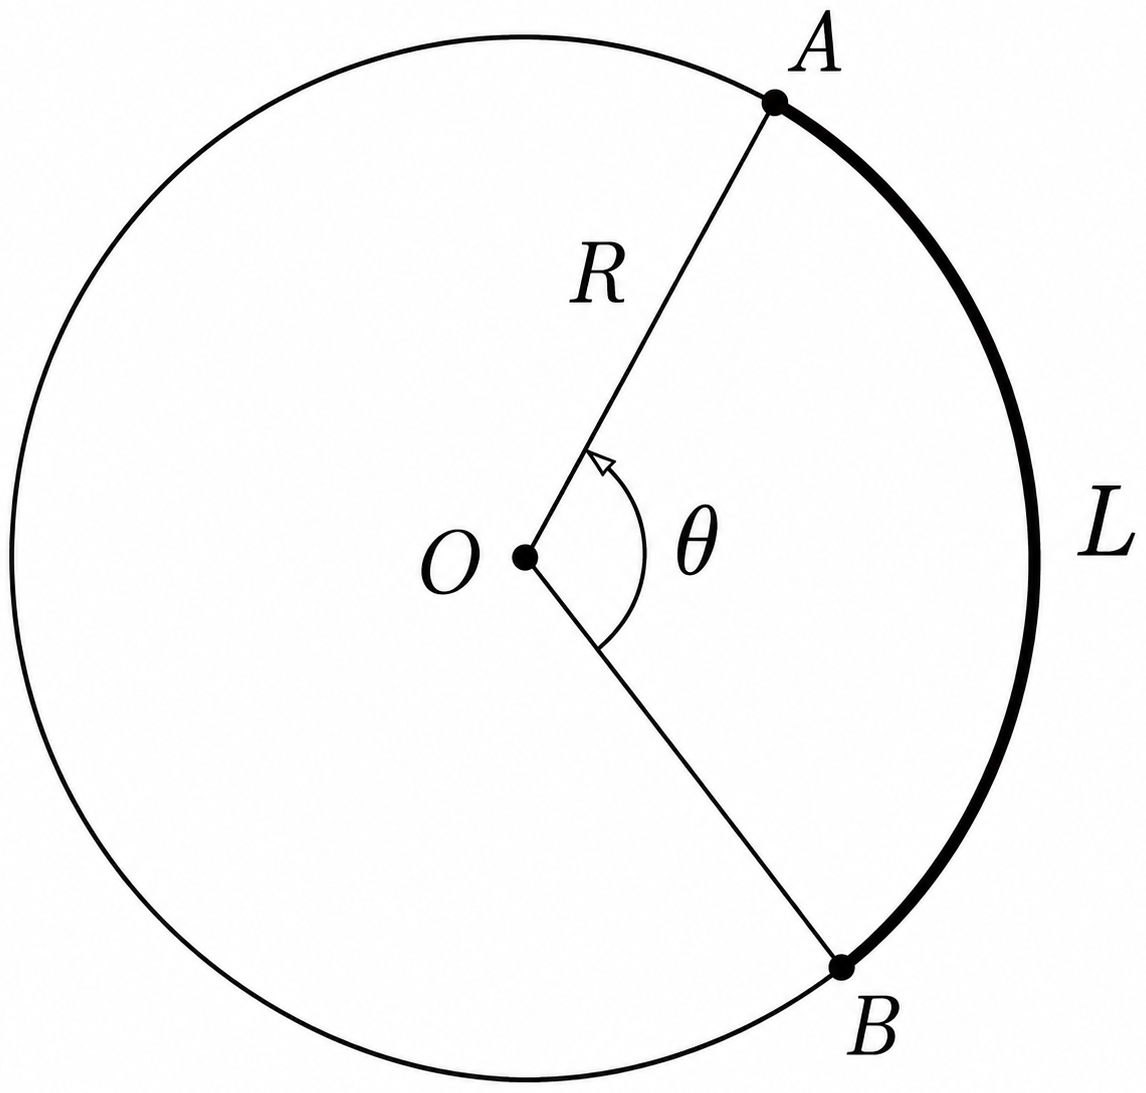
\includegraphics[width=0.4\textwidth]{circular_arc.png}
    \caption{Circle of radius $R$ and circular arc of length $L$ as seing by an angle of $\theta$.}
    \label{circarc}
\end{figure}

\ni
Following Fig.\,\ref{circarc} it is readily seen that the arc length $L$ of an arc of a circle with radius $R$ and central angle $\theta$, measured in radians, follows from the fact that the ratio between the arc length and the circumference of the circle is equal to the ratio between the central angle and the full angle $2 \pi$, mathematically
\be
\frac{L}{2\pi R} = \frac{\theta}{2\pi}.
\ee
One obtains $L = r\theta$. If the same angle is measured in degrees and denoted by $\theta^{\text{(deg)}}$, then
\be
\theta = \frac{\pi}{180} \theta^{\text{(deg)}}.
\ee
Therefore, the arc length $L = r\theta$ can also be written as
\be
L = \frac{\pi}{180} R \theta^{\text{(deg)}}.
\label{eq1}
\ee
The data consisting only of radii and central angles is not sufficient to determine the total length unless the geometric configuration specifies which arc of each circle contributes to the curve. For each circle, the effective angle is either the given central angle or its explementary angle. The geometric configuration of the problem imposes an essential subtlety: the arcs that form the line $AB$ do not correspond directly to the given central angles, but rather to the outer portions of the circles. Consequently, for each circle, the relevant angle must be replaced by its explementary angle $\alpha$ defined by
\be
\alpha_i = 2\pi - \theta_i.
\ee
Applying this transformation to the circles with centers $O_1, O_2, O_3, O_5$ and keeping the same interior angle for the circle with center $O_4$ results in the following set of angles that should be used for the calculus of the total length of $AB$ $\{270^\circ, 288^\circ, 225^\circ, 120^\circ, 255^\circ\}$.
The total length $L_{AB}$ of the line $AB$ from the chain of circles in Fig.\,\ref{fig:geometric-configuration} is then obtained by the summation of all of the arcs considering Eq.\,\eqref{eq1}
\be
L_{AB} = \frac{\pi}{180} \left(18 \cdot 270 + 35 \cdot 288 + 24 \cdot 225 + 36 \cdot 120 + 48 \cdot 255 \right).
\ee
Hence, the final answer for the total length or the line $AB$ is
\be
L_{AB} = 205\pi.
\ee
Thus concluding the solution to the problem.
\end{proof}

\ni
Table~\ref{tab:data} summarizes the numerical data required for the computation of the length of the curve $AB$. For each circle, the table lists the radius $R_i$, the angle $\theta_i$ given in the statement, the corresponding explementary angle $\alpha_i$, the angle effectively used in the arc-length formula, and the resulting contribution $L_i$. The fourth circle is the only case in which the given angle $\theta_i$ is used directly; in the remaining cases, the relevant arcs are determined by the explementary angles $\alpha_i$. 
\begin{table}[ht]
\centering
\caption{Data used in the computation of the length of $AB$.}
\label{tab:data}
\begin{tabular}{c c c c c c}
\hline
Center & $R_i$ (cm) & $\theta_i$ & $\alpha_i$ & Angle used & $L_i$ \\
\hline
$O_1$ & $18$ & $90^\circ$  & $270^\circ$ & $\alpha_i$ & $27\pi$ \\
$O_2$ & $35$ & $72^\circ$  & $288^\circ$ & $\alpha_i$ & $56\pi$ \\
$O_3$ & $24$ & $135^\circ$ & $225^\circ$ & $\alpha_i$ & $30\pi$ \\
$O_4$ & $36$ & $120^\circ$ & $240^\circ$ & $\theta_i$ & $24\pi$ \\
$O_5$ & $48$ & $105^\circ$ & $255^\circ$ & $\alpha_i$ & $68\pi$ \\
\hline
\multicolumn{5}{l}{} & $205\pi$ \\
\hline
\end{tabular}
\end{table}


\section{Generalization}

The same reasoning applies to any finite chain of $N$ tangent circles whose contributing arcs are known from the geometric configuration. Let the circles have radii $R_1, R_2,\ldots, R_N$, and let the corresponding central angles given in the statement be $\theta_1, \theta_2, \ldots, \theta_N$. For each circle, the arc contributing to the curve $AB$ may be either the arc subtended directly by $\theta_i$ or the arc subtended by its explementary angle
\be
\alpha_i = 2\pi-\theta_i,
\ee
when the angles are measured in radians. Let $\mathcal{I}_{\theta}$ denote the set of indices for which the arc used is the one associated with the given angle $\theta_i$, and let $\mathcal{I}_{\alpha}$ denote the set of indices for which the arc used is the explementary arc associated with $\alpha_i$. These two sets form a partition of the index set:
\be
\mathcal{I}_{\theta}\cup \mathcal{I}_{\alpha}=\{1,2,\ldots,N\},
\qquad
\mathcal{I}_{\theta}\cap \mathcal{I}_{\alpha}=\varnothing.
\ee
Therefore, the total length of the curve $AB$ is given by the expression
\be
L_{AB} = \sum_{i\in\mathcal{I}_{\theta}} R_i\theta_i 
+ \sum_{i\in\mathcal{I}_{\alpha}} R_i\alpha_i.
\ee
Since $\alpha_i = 2 \pi - \theta_i$, this can also be written as
\be
L_{AB} = \sum_{i\in\mathcal{I}_{\theta}} R_i\theta_i
+ \sum_{i\in\mathcal{I}_{\alpha}} R_i(2\pi-\theta_i).
\ee
If the angles are given in degrees, then the effective angle used for each arc is
\be
\beta_i^{\mathrm{(deg)}} =
\begin{cases}
\theta_i^{\mathrm{(deg)}}, & i\in\mathcal{I}_{\theta},\\[4pt]
360^\circ-\theta_i^{\mathrm{(deg)}}, & i\in\mathcal{I}_{\alpha}.
\end{cases}
\ee
Thus, the total length becomes
\be
L_{AB} = \frac{\pi}{180} \sum_{i=1}^{N} R_i\beta_i^{\mathrm{(deg)}}.
\ee
Equivalently,
\be
L_{AB} = \frac{\pi}{180} \left[ \sum_{i\in\mathcal{I}_{\theta}}R_i\theta_i^{\mathrm{(deg)}} + \sum_{i\in\mathcal{I}_{\alpha}}R_i \left(360^\circ-\theta_i^{\mathrm{(deg)}}\right)
\right].
\ee
For the particular problem analyzed in the previous section of this work
\be
N=5,
\qquad
\mathcal{I}_{\theta}=\{4\},
\qquad
\mathcal{I}_{\alpha}=\{1,2,3,5\}.
\ee

\section{Conclusion}

The problem discussed in this work illustrates how an elementary question in plane geometry can lead to a generalization. Starting from a specific configuration of tangent circles, we showed that the length of the curve $AB$ is obtained by identifying, for each circle, the effective arc that contributes to the curve. This point is essential: the numerical data alone, consisting of radii and central angles, do not determine the answer unless the geometric configuration specifies whether the relevant arc is associated with the given central angle or with its explementary angle.

\begin{thebibliography}{9}

\bibitem{dolce-pompeo}
DOLCE, Osvaldo; POMPEO, José Nicolau. \textit{Fundamentos de Matemática Elementar: Geometria Plana}. Vol.~9, 7th ed. São Paulo: Atual Editora, 1993.

\end{thebibliography}

\end{document}